\chapter{Structural Graphics in GSAS-II}\label{Chap:structureplotting}

GSAS-II provides structural visualization as part of the Phase data tree item. This chapter introduces some of the capabilities offered there. 
While this can be used for publication-quality graphics and there may well be things that GSAS-II's molecular visualization does that would be hard to duplicate in other software, it should also be noted that there are many other crystallographic graphics packages that may be better for many tasks. These include the free Mercury and Vesta programs, as well as CrystalMaker and Diamond. However, where GSAS-II's graphics are most useful is in its integration into the structure completion and refinement process, which will be the focus of what I present here. Before going into the GUI for structure visualization, it is worthwhile to first describe what is actually displayed. 
For the following discussion, I will label the axes of the screen as having x horizontal, y as vertical and z as coming out from the screen.

GSAS-II uses OpenGL graphics to display the structure in three dimensions. Well, since the structure is displayed on a two dimensional screen, it is really a 2D drawing, but it includes perspective and Z-clipping (which hides objects that are too ``close'' to you as a viewer) and can be rotated in space, which allows our brains to interpret what we are seeing in 3D. I still find it somewhat amazing that this ``3D graphics'' technology, that was at first only available to me on a nearly desk-sized \$60,000 Silicon Graphics computer (that a previous employer pushed me into learning to use) is now available on a mobile phone. 

Dragging the mouse will change our view of the structure. Dragging the mouse up and down using the left mouse button rotates around screen x axis, and dragging right and left rotates around screen y.  The middle mouse button rotates our view of the structure around the screen z axis. The right mouse button translates the view point in the plane of the screen. To move the view point in three dimensions, rotate around screen x or y and then translate again. If you have a mouse wheel, rotating that changes the ``camera position'', which can be thought of as moving the structure closer or farther from where it is viewed. This can also be changed from the Draw Opts tab. The structure rotates around a point that GSAS-II calls the ``view point''.

The view point is always placed in the center of the graphics window. If the ``Show view point'' option is set as on in the ``Draw Options'' tab (this is the default), it is drawn with 1 $\mathring{\text{A}}$ lines along the \textit{a}, \textit{b} and c, directions, with the lines colored red, green and blue, respectively. The unit cell, when outlined, is also drawn with red, green and blue lines for the \textit{a}, \textit{b} and c,  axes, respectively. Colored lines are used for the lines starting from x=y=z=0  and the remaining lines are white.

To provide some orientation to the GUI, there are three tabs within each phase data tree item that all interact for visualization; they are the ``Atoms``, ``Draw Atoms'' and ``Draw Options,'' which will be discussed further in this chapter, but there are other tabs that can also influence what appears in the visualization. Here is a synopsis of all these phase tabs and their relevance to structure visualization:
\begin{itemize}
    \item Atoms: contains the atom positions and ADP values that are used for display
    \item  Draw Atoms: has the atoms that appear in the visualization. These are copies of the atoms from the Atoms tab, potentially with symmetry and unit cell translations applied.
    \item Draw Options: this contains settings and controls for visualization. 
    \item General: has settings for computation of Fourier maps (also see Chapter \ref{Chap:intextraction}), but the Draw Options settings will control how the Fourier map information is displayed.
    \item Map Peaks: has a list of peaks from Fourier maps; these are shown on the plot and may have distances displayed depending on the Draw Options settings.
    \item RB Models: Visualization can aid the process of defining a rigid body for a phase. The options shown on this tab control how rigid bodies are visualized. 
\end{itemize}

\section{Phase ``Atoms'' tab}
This data window shows the atoms in the current phase. This has the atom positions used to generate the visualization graphics, but no changes need to be made here to control those graphics. The only direct interaction between the graphics and this tab are that view point location on the plot can be utilized here. The ``Edit Atoms''/``Append view point'' menu command will place a H atom at whatever is the current view point location; this can then be changed to another element by clicking on the atom's Type entry. 

It is possible to select atoms in the Atoms table by clicking on the row entries, but nothing is done when a  selection is made in that way. However, if  the structure visualization is created from either the ``Draw Atoms'' or ``Draw Options'' tab, you then return to the ``Plot'' tab and finally, the plot window is made active by clicking on the window border or inside the window, and then by pressing the  ``n'' or ``p'' keys, one can advance the selection through the Draw Atoms atoms table (n forward, p backwards). When an atom is selected, that atom will be highlighted in the plot by changing the atom color to a bright green and the view point will be placed on that atom. 

Changes made to coordinate/ADPs in the Atoms list are not always propagated to the atom information in the  Draw Atoms tab, but the menu command ``Edit Atoms''/``Update draw atoms'' will update the information in Draw Atoms. 

\section{Phase ``Draw Atoms'' tab}\label{ref:atomchangeselection}
The information shown on the Draw Atoms tab is a list of atoms that may include symmetry replicants of atoms in the Atoms tab. There is an extensive list of menu commands that determine how atoms are added to this list, as will be discussed further below. Note that the only settings that can be changed for each atom in this list are entries in the columns labeled Style, Label, and Color. Note that these settings are independent. The values for these settings can be changed one at a time, by clicking on the appropriate box in that column, or you can use the  ``Atom style'', ``Atom label'', and/or ``Atom color'' menu commands in the ``Edit Figure'' menu. This will change the value for all selected atoms, or, if no atoms are selected, you will be given a window to select atoms. Also, it is possible to change the values for one or more atoms by selecting them and using a right click, or by double-clicking on the column label. 

\subsection{Atom selection}
Atoms may be selected in the table by clicking on the row label (to the left). 
If the shift key is help down, ranges of atoms can be selected and if the alt key (cmd on Mac) is held down, individual atoms can be added or removed from the selection list.  
Alternately, the ``Edit Figure''/``Select from list'' menu command can be used and you will be given a window to select atoms. Finally, with the plot window active, one can advance the selection through the Draw Atoms atoms table by pressing on the ``n'' or ``p'' keys. 
Note that when atoms are selected in the table, their color is changed to a bright green.  This can be helpful when trying to understand the structure difference between the crystallographically different atoms with the same element type. When the ``n'' or ``p'' keys are used for selection, the view point will be placed on that atom. 

\subsection{Style options}
The style setting dictates how atoms are displayed. The options are:
\begin{itemize}
    \item lines: Here thin lines are used to connect atoms. If an atom has no bonds, it will not be directly visible.
    \item vdW balls: This draws the atoms as van der Waals spheres that are intended to be space-filling. Bonds are not drawn to connect atoms  that are drawn as van der Waals spheres. There is a scaling factor for the size used for van der Waals spheres that can be adjusted on the Draw Options tab.
    \item sticks: Like the lines mode, atom positions are not drawn directly, but bonds between atoms are shown. However, in this mode, cylinders are used to show bonds. The thickness of the cylinder can be adjusted on the Draw Options tab.
    \item balls \& sticks: This places spheres at the positions of selected atoms and also draws bonds as cylinders between atoms. The same adjustment on the Draw Options tab for the thickness of the ``sticks'' cylinders also changes the bonds here, but there is a separate scaling factor for the ball size on the Draw Options tab.
    \item ellipsoids: This option will draw atom sizes as proportional to the APD values. Ellipsoids are used for atoms where anisotropic $\rm U_{ij}$ values are refined and spheres are used where $\rm U_{iso}$ is selected. There is an ellipsoid probability factor on the Draw Options tab.
    \item polyhedra: This option draws solids around bonded atoms, The color of the solid is determined by the central atom. 
\end{itemize}

\subsection{Label options}
Labels can be placed at atom positions, but these labels may be hidden by spheres or ellipsoids if one of these options has been selected. Dropping the scaling/probability factor down will reveal the labels. The choices for label are:
\begin{itemize}
    \item type, where the label is the element type, 
    \item name, where the label is the name specified for the atom on the``Atoms'' tab.
    \item number, where the number listed by the sequence on the``Draw Atoms'' tab. Note that this and atom selection are the ways to distinguish between symmetry replicants of atoms.  
\end{itemize}
If the label option is left blank (the default), no label is provided for that atom. 

\subsection{Atom colors}
The default atom color is set from the value for the element type shown on the General tab. The default can be changed there. When any of the methods given in section \ref{ref:atomchangeselection} is used, a dialog will be presented for color selection, but the nature of this dialog will be determined by the operating system on your computer. 

% \subsection{Atom Bonding Settings}

\subsection{Adding to the Draw Atoms}
When the Draw Atoms tab is first selected, the atoms in the asymmetric unit, as listed on the Atoms tab, are placed into this list. If all the atoms are deleted from the Draw Atoms list, the contents are reset to the atoms in the asymmetric unit. There are a number of commands provided that allow you to expand the number of atoms in the Draw Atoms list. Note that they will all remove duplicate atoms, so you do not need to worry about an operation that will duplicate atoms that are already in the list. 
\begin{itemize}
    \item Fill unit cell: The menu command that I use more than any other is ``Fill unit cell''. This will take the selected atoms (or ask if none are selected) and find all the symmetry replicants of those selected atoms that are located in the unit cell and add them to the Draw Atoms list.
    \item Fill CN-sphere: This will add the atoms directly bonded to the selected atoms. 
    \item Add sphere of atoms: Here one designates one or more ``origin'' atoms and a sphere of a specified radius is searched for atoms that are within that distance. You can select what type of atoms will be searched. 
    \item Add atoms: This command allows one to apply a specified symmetry transformation to a set of atoms. Note that the selected symmetry operation is applied directly to the position of the atom as it appears in the Draw Atoms listing. A good way to generate two unit cells worth of atoms is to first use the ``Fill unit cell'' menu command and then select all atoms in the table and use the ``Add atoms'' command. Here use the X, Y, Z symmetry operator and do not force to unit cell and then select the a neighboring unit cell [(1,0,0) or (0,1,0) or (0,0,1) or (-1,0,0) or (0,-1,0) or (0,0,-1)]. Repeat the  ``Add atoms'' command to expand further. While I cannot provide examples, I am sure there are many other ways this command could be used to create useful sets of atoms to plot. 
    \item Transform atoms: This command works very similarly to the  ``Add atoms'' command except that instead of adding the generated positions, the existing atoms in the Draw Atoms list are replaced by the generated positions. If you have an asymmetric unit that has atoms outside the unit cell, but want to obtain the unit cell contents, use this command with the option ``Force to unit cell'' set as ``yes,'' either before or after the ``Fill unit cell'' menu command. 
    \item Complete molecule: This is most useful for structures with discrete molecules, rather than structures that create infinite networks, but sometimes can be useful for the latter by not including linking atoms (for example metal ions in MOFs). What it does is use the ``Fill CN-sphere'' command on the selected atoms and then applies the ``Fill CN-sphere'' command on the atoms that have been generated. This command will fill out the bonding in molecular fragments and then stop once all the atoms in the fragment have been located. If accidentally launched on an infinite framework, it will keep discovering new bonded and would never stop, which is why the command has a limit for how many iterations will be applied in the command and the maximum number of atoms that will be allowed. 
\end{itemize}

\subsection{Other Actions from Draw Atoms}
Here are some of the other actions that can be performed from the Draw Atoms tab from the ``Edit Figure'' menu:
\begin{itemize}
    %\item Edit atom radii
    \item Set view point: the view point is set to the average position of the selected atoms. Works nicely with a single atom or a group of atoms. 
    \item Update draw atoms: Usually the information in the Draw Atoms list is synchronized to changes in the Atoms list, but should that fail, this command will update the Draw Atoms coordinates/ADP values. 
    \item Load selected atoms: This can be used to copy selected atoms from the Atoms list to the Draw Atoms list. This is not commonly needed, but might be used after an atom is accidentally deleted from the Draw Atoms list or has been transformed, but is wanted at the original position again. 
    \item Randomized Action: This selects atoms in a randomized order and gives you the opportunity to do something you have chosen to those selected atoms. As an example, if you want to convert a structure that has vacancies noted by partial occupancy to an atomistic model, you might want to delete a percentage of those atoms. With this command, you could select all the generated symmetry replicants of that atom and then delete the first \textit{n}\% of those atoms. 
\end{itemize}

This action can be performed from the Draw Atoms tab from the ``Compute'' menu:
\begin{itemize}
    \item Create void map: this sweeps through the unit cell on the specified grid spacing and locates points where there are no atoms (as determined by their space-filling radius) within a specified distance. Blue dots (actually small cubes) are then placed at those locations where there are no atoms. The default is to create small blue dots that can be somewhat hard to see against a black background on some monitors, but the GUI allows them to be made brighter or to change the size or color.\index{void map}
\end{itemize}
\subsection{Window keystrokes}
These commands require that the plot window be active (by clicking on the graphics window border or inside the window).
\begin{itemize}
    \item c: pressing the ``c'' key will reset the view point to its default value of ($\frac12, \frac12, \frac12$).
    \item n: will select the next atom in the Draw Atoms list
    \item p: will select the previous atom in the Draw Atoms list
    \item +: The ``+'' key the view point along the screen z-axis, moving the view point in the direction towards the viewer, The structure will appear to move away as the plot is centered on the new view point. 
    \item -: The ``-'' key moves the view point along the screen z-axis, moving the view point in the direction away the viewer, The structure will appear to towards the viewer.  
\end{itemize}

\section{Phase ``Draw Options'' tab}
The GUI for the Draw Options tab is divided in sections. The top section has values that determine how the plot is displayed, as shown in Fig. \ref{fig:DrawOpts1}. Many of these values were discussed above. 
\begin{figure}
    \centering
    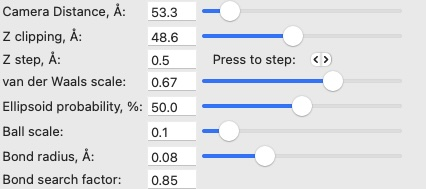
\includegraphics[width=0.5\linewidth]{figures/PlotOptions1.jpg}
    \caption{Top portion of the data window contents, when the Draw Options tab is selected for a phase data tree entry. These parameters determine how the plot is drawn.}
    \label{fig:DrawOpts1}
\end{figure}

The second section is shown in Fig. \ref{fig:DrawOpts2}. This mostly is used to manipulate the contents and orientation of the graphics. The view direction is the real space axis that points from the view point to you. It will be updated as the plot is rotated. Alternately one can type into that box, where entering ``1 1 1'' will have you view down the body diagonal for the cell. Likewise the view point coordinates can be seen or changed here as well. As a way to explore the structure, one can place the view point in a particular location. Depending on the distances set for the three options, symmetry replicants for Fourier map points and atoms will be shown if within the specified distance. Likewise, distances to atoms or map points to the view point can be labeled on the plot. The final options determine if different plot options are included in the plot. The ``Fade sym equivs?'' option will make the atoms in the asymmetric unit stand out with respect to the symmetry-generated replicants. 
\begin{figure}
    \centering
    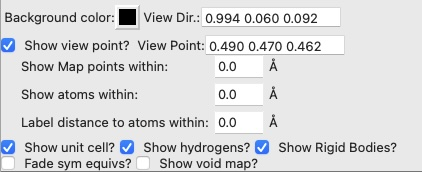
\includegraphics[width=0.5\linewidth]{figures/PlotOptions2.jpg}
    \caption{Middle portion of the data window contents, when the Draw Options tab is selected for a phase data tree entry. These parameters determine how the plot is viewed and what is included.}
    \label{fig:DrawOpts2}
\end{figure}

The section of the window shown in Fig. \ref{fig:DrawOpts3} allows you to draw a plane or line on the plot, to help visualize directions. Note that the (0,0,1) plane is perpendicular to \textit{c} at z=0, while the (0,0,5) plane is parallel but has z=0.2. The phase shift can be also used to displace the planes and the stack option shows all the planes within the unit cell. Likewise, the ``line from view point'' will draw a line in a particular direction. \begin{figure}
    \centering
    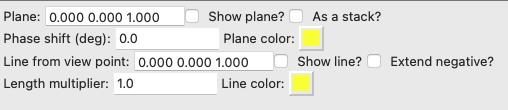
\includegraphics[width=0.5\linewidth]{figures/PlotOptions3.jpg}
    \caption{Top portion of the data window contents, when the Draw Options tab is selected for a phase data tree entry. These parameters determine how the plot is viewed.}
    \label{fig:DrawOpts3}
\end{figure}

When a Fourier map is computed, an extra section appears in the data window, as shown in  in Fig. \ref{fig:DrawOptsF}. These options affect how Fourier maps and peaks from that map are displayed and are discussed in section \ref{ref:FourierViewOpts}.

\begin{figure}
    \centering
    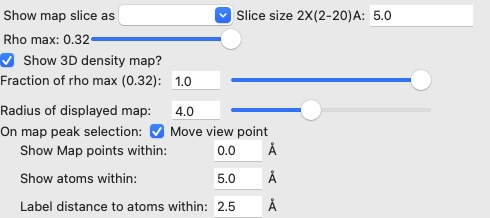
\includegraphics[width=0.5\linewidth]{figures/PlotOptionsF.jpg}
    \caption{Top portion of the data window contents, when the Draw Options tab is selected for a phase data tree entry. These parameters determine how the plot is viewed.}
    \label{fig:DrawOptsF}
\end{figure}
